% This is "sig-alternate.tex" V1.9 April 2009
% This file should be compiled with V2.4 of "sig-alternate.cls" April 2009
%
% This example file demonstrates the use of the 'sig-alternate.cls'
% V2.4 LaTeX2e document class file. It is for those submitting
% articles to ACM Conference Proceedings WHO DO NOT WISH TO
% STRICTLY ADHERE TO THE SIGS (PUBS-BOARD-ENDORSED) STYLE.
% The 'sig-alternate.cls' file will produce a similar-looking,
% albeit, 'tighter' paper resulting in, invariably, fewer pages.
%
% ----------------------------------------------------------------------------------------------------------------
% This .tex file (and associated .cls V2.4) produces:
%       1) The Permission Statement
%       2) The Conference (location) Info information
%       3) The Copyright Line with ACM data
%       4) NO page numbers
%
% as against the acm_proc_article-sp.cls file which
% DOES NOT produce 1) thru' 3) above.
%
% Using 'sig-alternate.cls' you have control, however, from within
% the source .tex file, over both the CopyrightYear
% (defaulted to 200X) and the ACM Copyright Data
% (defaulted to X-XXXXX-XX-X/XX/XX).
% e.g.
% \CopyrightYear{2007} will cause 2007 to appear in the copyright line.
% \crdata{0-12345-67-8/90/12} will cause 0-12345-67-8/90/12 to appear in the copyright line.
%
% ---------------------------------------------------------------------------------------------------------------
% This .tex source is an example which *does* use
% the .bib file (from which the .bbl file % is produced).
% REMEMBER HOWEVER: After having produced the .bbl file,
% and prior to final submission, you *NEED* to 'insert'
% your .bbl file into your source .tex file so as to provide
% ONE 'self-contained' source file.
%
% ================= IF YOU HAVE QUESTIONS =======================https://github.com/Boidkan/Senior_seminar_templates.git
% Questions regarding the SIGS styles, SIGS policies and
% procedures, Conferences etc. should be sent to
% Adrienne Griscti (griscti@acm.org)
%
% Technical questions _only_ to
% Gerald Murray (murray@hq.acm.org)
% ===============================================================
%
% For tracking purposes - this is V1.9 - April 2009

\documentclass{sig-alternate}
\usepackage{color}


%%%% User-defined macros
\newcommand{\lam}{\lambda}
\newcommand{\mycomment}[1]{\textcolor{red}{#1}}
%%%%% Uncomment this line (and comment the previous one)
%%%%% to remove all comments
%%%%% NOTE: comments still occupy a line even if invisible;
%%%%% Don't write them as a separate paragraph
%\newcommand{\mycomment}[3]{}
%\linespread{2}
\begin{document}

%
% --- Author Metadata here ---
\conferenceinfo{UMM CSci Senior Seminar Conference, April 2014}{Morris, MN}
%\CopyrightYear{2007} % Allows default copyright year (200X) to be over-ridden - IF NEED BE.
%\crdata{0-12345-67-8/90/01}  % Allows default copyright data (0-89791-88-6/97/05) to be over-ridden - IF NEED BE.==
% --- End of Author Metadata ---

\title{Applying Genetic Programming to \\ Bytecode and Assembly}
%\subtitle{[Extended Abstract]
%
% You need the command \numberofauthors to handle the 'placement
% and alignment' of the authors beneath the title.
%
% For aesthetic reasons, we recommend 'three authors at a time'
% i.e. three 'name/affiliation blocks' be placed beneath the title.
%
% NOTE: You are NOT restricted in how many 'rows' of
% "name/affiliations" may appear. We just ask that you restrict
% the number of 'columns' to three.
%
% Because of the available 'opening page real-estate'
% we ask you to refrain from ElenaSampleputting more than six authors
% (two rows with three columns) beneath the article title.
% More than six makes the first-page appear very cluttered indeed.
%
% Use the \alignauthor commands to handle the names
% and affiliations for an 'aesthetic maximum' of six authors.
% Add names, affiliations, addresses for
% the seventh etc. author(s) as the argument for the
% \additionalauthors command.
% These 'additional authors' will be output/set for you
% without further effort on your part as the last section in
% the body of your article BEFORE References or any Appendices.
\numberofauthors{1} %  in this sample file, there are a *total*
% of EIGHT authors. SIX appear on the 'first-page' (for formatting
% reasons) and the remaining two appear in the \additionalauthors section.
%
\author{
% You can go ahead and credit any number of authors here,
% e.g. one 'row of three' or two rows (consisting o
% and a second row of one, two or three).
%
% The command \alignauthor (no curly braces needed) should
% precede each author name, affiliation/snail-mail address and
% e-mail address. Additionally, tag each line of
% affiliation/address with \affaddr, and tag the
% e-mail address with \email.
%
% 1st. author
\alignauthor
Eric C. Collom \\
\affaddr{University of Minnesota, Morris} \\
\email{coll0474@morris.umn.edu}
}

\maketitle
\begin{abstract}
Traditional genetic programming (GP) has not yet been able to evolve entire programs at the source code level. Instead only small sections within the programs are usually evolved. Evolving programs in either bytecode or assembly language is a method that solves this problem. This paper provides an overview of applying genetic programming to Java bytecode and x86 assembly to solve problems. Two examples of how this method can be implemented will be explored. We will explore how they evolve bytecode and assembly and discuss their experimental results.
\end{abstract}


\keywords{evolutionary computation, x86 assembly code, Java bytecode, FINCH, automated bug repair}

\section{Introduction}
GP is a set of techniques used to automate computer problem solving. This is done by evolving programs with an evolutionary algorithm (EA) that imitates natural selection in order to find a solution. Traditional GP has been used mostly to evolve only specific parts of programs and not full-fledged programs themselves. This is because traditionally we have to understand the structure of the program being evolved. An EA is usually designed for a specific program with knowledge about how the program works. Being able to evolve an entire program without knowing its structure would allow for more flexibility in GP. Evolving bytecode and assembly, instead of source code, is a method that allows for this flexibility. This is possible because bytecode and assembly languages are less restrictive syntactically than source code. We discuss this issue further in Section 3.\par 

Orlov et al.,~\cite{FINCH2:2009} propose a method of applying GP to full-fledged programs that only requires a program to be compiled to Java bytecode. Once in Java bytecode an EA is applied to the program to solve the desired problem. Schulte et al.,~\cite{Assembly:2010} also apply a similar method with both Java bytecode and the x86 assembly family.

These methods are important because they show that evolving entire programs is possible. This is useful since once the EA has been created there is little modification that has to be done to it to evolve different programs. Also, the structure of the program being evolved does not have to be known or modified.\par

	This paper will examine how both Orlov et al.,~\cite{FINCH:2011} and Schulte et al.,~\cite{Assembly:2010} apply GP to solve programs in Java bytecode and x86 assembly. We will show that this methodology is feasible in Section 6. Orlov et al.,~\cite{FINCH:2011} focused on evolving simple programs as a whole while Schulte et al.,~\cite{Assembly:2010} focused on automated bug repair in programs.\par
	
This paper is organized as follows: Section 2 covers the background needed for understanding that application of GP to bytecode and assembly. It contains information on Evolutionary Computation (EC), x86 assembly, and Java bytecode. Section 3 describes the benefits of evolving assembly and bytecode. Section 4 discusses how Orlov, et al.,~\cite{FINCH:2011} evolved Java bytecode. Similarly, in Section 5 we discuss how Schulte, et al.,~\cite{Assembly:2010} evolved both x86 assembly and Java bytecode. In section 6, we report some of the problems solved by \cite{FINCH:2011} and \cite{Assembly:2010} in applying GP to bytecode and assembly. Section 7 will address possible future work and ideas.  
	
	

\section{Background}


This section explores the components of evolutionary computation (EC) and GP. x86 and Java bytecode are will also be discussed. Additionally, we will analyze basic details of the Java Virtual Machine (JVM).
\subsection{Evolutionary Computation}
\begin{figure}
\centering
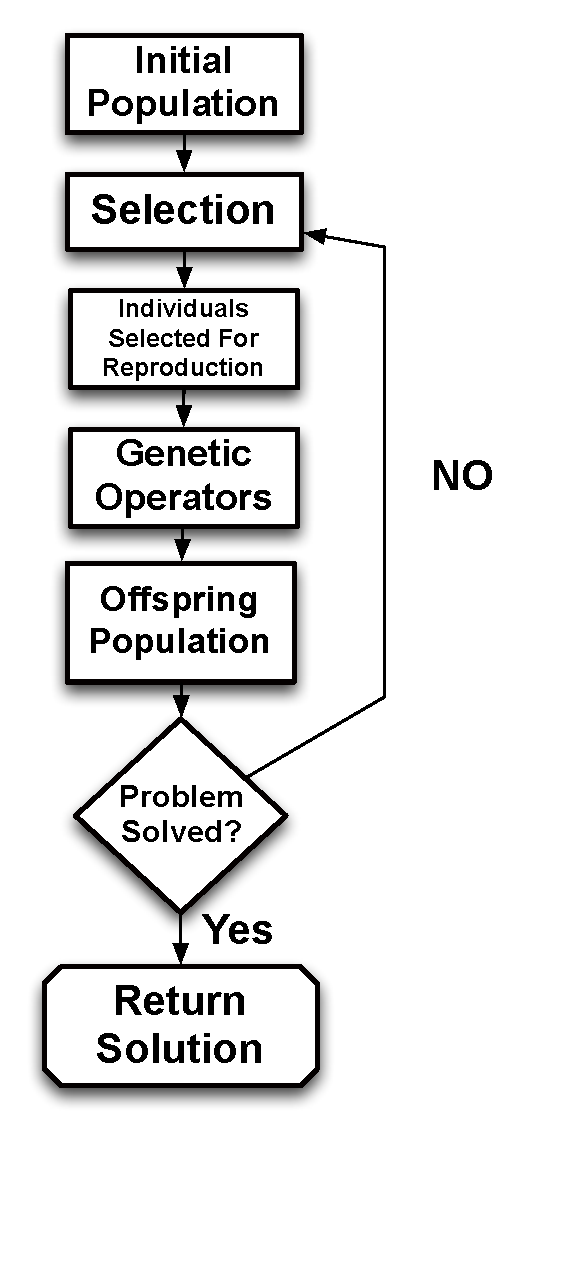
\psfig{file=ECdiagram.pdf,height=3in}

\caption{The process of of Evolutionary Computation}
\label{ECdiagram}
\end{figure}


EC is a field of computer science and artificial intelligence that is loosely based on evolutionary biology. EC imitates evolution through continuous optimization in order to solve problems. Optimization in EC is the selection of the best individual within a population. What an individual is depends on the problem being solved. For example, It can be a string of bits, a lisp tree, or an object. For clarity, in this paper the individuals will be programs.\par 

Figure~\ref{ECdiagram} shows the process of evolution in EC. An initial population of individuals is taken and a selection process is done to choose the most fit individuals who are then taken and modified with genetic operators that imitate procreation between two individuals. A check is then done to see if any individuals from the population solve the desired problem. If not, the process of evolution is repeated. If the problem is solved the individual with the best solution is returned.\par

	GP is a tool that uses the EC process to evolve programs. GP evolves an initial population of programs either until the desired solution to the problem is found or a specified number of generations is reached. The fitness of each individual is the deciding factor on how likely it is to be chosen for evolution. The fitness is a value, usually numerical, that indicates how well an individual solves the specific problem. For the research discussed in this paper a higher fitness indicates a more fit individual. The selection of individuals for procreation is done through tournament selection. A certain number of individuals are chosen for a simulated competition and the individual with the highest fitness wins. That individual is then used for procreation.\par 
		
	One way procreation is simulated in GP is through the genetic operator called crossover. Crossover is the process of taking two individuals and extracting a section of code from one and then replacing it with a section from the other program to form an offspring which is a new program.\par 
	
	Mutation is another genetic operator that is used to produce offspring. Mutation takes a program and randomly changes a section. Mutation can be used along with crossover to produce offspring.


\subsection{x86 Assembly \& Java Bytecode}

\begin{figure}
\centering
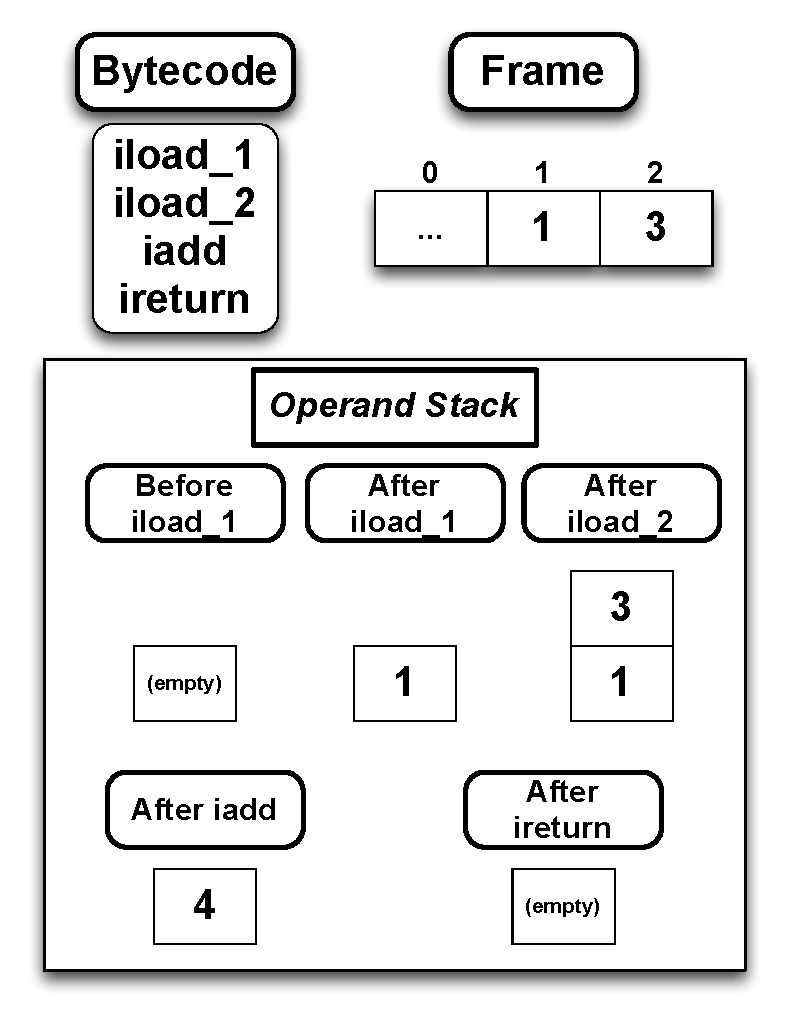
\psfig{file=stackBytecode.pdf,height=2.5in}

\caption{In this example we are assuming that the frame already contains the local variables 1 and 3 to retain simplicity. This Java bytecode sequence pushes two numbers to the stack and adds them and returns the value.}
\label{stack}
\end{figure}


Throughout the rest of this paper the term \textit{instruction-level code} will be used when referring to Java bytecode and x86 assembly as one unit. Instruction-level code consist of operation codes (opcodes) which are one byte in length. However, some opcodes that take parameters are multiple bytes in length~\cite{JavaBytecode:2014,x86tomachine:2013}.

\subsubsection{X86}
x86 is a family of backward compatible low-level programming languages~\cite{x86assembly:2014} created by Intel and designed for specific computer architectures. They are designed to only run on certain physical machines. 

\subsubsection{ Bytecode and the JVM}
Java bytecode ``is [an] intermediate, platform-independent representation''~\cite{FINCH2:2009} of Java source code. However, ``implementors of other languages can turn to the Java Virtual Machine as a delivery vehicle for their languages''~\cite{JVMspec:2013}. A few examples of languages with which this has been done are Scala, Groovy, Jython, Kawa, JavaFx Script, Clojure, Erjang, and JRuby.

The JVM executes bytecode through a stack-based architecture. Each JVM thread has a private stack which can only be popped and pushed to. Each private stack stores frames. Each frame contains an array of local variables, its own operand stack, and a reference to the class of the current method\footnote{It is a reference to the run time constant pool of the class of the current method. More details can be found in chapter 2.5.5 of ~\cite{JVMspec:2013}}. A new frame is created when a method is invoked. When a method is done executing, the frame is destroyed~\cite{Oracle:2013}. Only the frame of the current executing method within a thread can be active at any time. Popping from a stack is simply removing the top element while pushing is putting an element on top of the stack.

Figure~\ref{stack} is a simple example of what Java bytecode looks like and how the stack works. Each of the opcodes in Figure \ref{stack} contain the prefix \texttt{i} which stands for the primitive integer type. These opcodes can only manipulate integers. The prefix is followed by the operation to be executed.\par 

The opcodes that we will be examining in this paper are: \texttt{iconst\_n}, \texttt{istore\_n}, \texttt{iload\_n}, \texttt{iadd}, \texttt{isub}, and \texttt{ireturn}. \texttt{iconst\_n} produces an integer type of value \texttt{n} and pushes it on the stack. \texttt{istore\_n} pops the stack and saves that element value at index n on the frame. \texttt{iload\_n} takes the value of the element at index \texttt{n} on the frame and pushes it to the stack. \texttt{iadd} pops two elements from the stack, adds them and pushes the result to the stack. Similarly, \texttt{isub} pops two elements, subtracts the second element from the first element and pushes the result to the stack. \texttt{ireturn} simply pops the stack and returns that value.

In Figure, \ref{stack} when \texttt{iload\_1} is executed, it takes the element from the frame at index 1 and pushes it onto the stack. \texttt{iload\_2} does the same thing but with index 2. \texttt{iadd} pops two elements from the operand stack, which both must be of integer type, adds them and then pushes the result to the stack. \texttt{ireturn} simply pops the stack and returns that element. \mycomment{I feel I don't need this anymore. It is a bit repetitive. Should I just explain in more general terms what figure 2 is doing without going into detail how each opcode works? Or should I just forget about that and just have the explanation in the caption?}



\begin{figure}
\centering
{\tt
\begin{verbatim}
float x;                    int x=7;
int y=7;                    float y;
if(y>=0){                   if(y>=0){
    x=y;                        y=x;
}else{                          x=y;
    x=-y;                   }
}                           System.out.println(z);
System.out.println(x);	
     
     (a)                      (b)

\end{verbatim}
}
\caption{Both (a) and (b) are valid code syntactically however only (a) is valid semantically.}
\label{semantics}
\end{figure}



\section{Instruction-level Code Benefits}

We encounter many problems when trying to evolve source code. It is extremely difficult to evolve an entire program due to source code syntactical constraints. Traditional GP has yet to take a whole program and evolve it. The structure of the program must be known and understood in order to design an EA for that problem. When an EA is designed, it is common to simply evolve expressions or formulae within the program~\cite{FINCH:2011}. Most of the program would already be written and remain the same after evolution. The EA has must know what it can evolve and its location. This limitation is due to the difficulty of dealing with semantic constraints in source code.

\subsection{Source Code Constraints}
There is a high risk of producing a non-compilable program when evolving programs at the source code level. This is due to the fact that high-level programming languages are designed to simplify reading and writing programs. Most high-level programming languages are defined by using grammars which are used to represent the syntax of the programming language~\cite{Oracle:2013,Assembly:2010}. The grammar does not represent the semantic constraints of a program. It does not capture the languages type system, variable visibility and accessibility, or other constraints ~\cite{FINCH:2011}. For example, in Figure~\ref{semantics} both \ref{semantics}(a) and \ref{semantics}(b) comply with the syntactical rules of Java but 3(b) breaks the semantic rules and thus is illegal code. In \ref{semantics}(b), variable \texttt{y} is uninitialized before the test in the if statement, assigning \texttt{y} to \texttt{x} violates a type constraint, and variable \texttt{z} is not defined. In order to write a program to evolve source code we would have to deal with all these constraints. While this task is possible, it would require creating a full-scale compiler to check for these semantic constraints. Thus, it is easier to evolve instruction-level code. \par

Instruction-level code consists of a smaller set of instructions~\cite{Assembly:2010}. It is simpler syntactically and there are less semantic constraints to violate. Thus, there is a lower risk of producing a noncompilable program during evolution and it is easier to design an EA that deals with the semantic constraints.

\subsection{Flexibility  for Individuals}

When evolving instruction-level code the program does not have to be ``intentionally written for the purpose of serving as an EA representation''~\cite{FINCH2:2009}. Furthermore, an understanding of the structure of the program is not required. The only requirement is that it can be compiled to instruction-level code~\cite{FINCH2:2009, Assembly:2010}. The EA does not have to focus on a specific part of the program in order to perform evolution. Understanding of the desired output, rather than input, is more important when designing the EA. A program that is being evolved stays as is and the EA goes through minor modifications to fit the problem being solved. The EA has to be given a fitness function in order to attempt to find a desirable individual. It also needs to know what genetic operators are needed as well as the desired number of generations. Depending on the program being evolved, a growth limit, on the individuals, might have to be enforced. For example, Orlov et al.,~\cite{FINCH:2011} enforced a growth limit when performing crossover on code so that the programs would not become too large.

A huge benefit that comes from evolving instruction-level code is that the initial program being evolved does not have to contain a great deal of code. This is partially due to the fact that a small program can contain a large amount of instructions-level code~\cite{Assembly:2010}. The EA can evolve a minimal amount of code into a full-scale working program.\par 

When evolving instruction-level code it is also possible to evolve a very focused area within the program; similar to how traditional GP is applied to source code. For example, Schulte et al.,~\cite{Assembly:2010} designed their EA to only evolve smaller areas of code and only made minor changes to the code as a whole. The resulting code would usually only have one line of code changed. Since they were evolving instruction-level code, they were able to fix bugs such as incorrect type declarations. This had not been possible in their earlier work done in source code~\cite{Forrest:2009}. 

\section{FINCH}
FINCH is a program developed by Orlov et al.,~\cite{FINCH2:2009,FINCH:2011} that evolves programs that have already been compiled into Java bytecode. FINCH uses two-point crossover to evolve Java bytecode. It takes two programs \texttt{A} and \texttt{B} and extracts sections $\alpha$ and $\beta$ respectively. It then takes section $\alpha$ and inserts it into where section $\beta$ used to be. It only selects an $\alpha$ that will compile after being inserted into \texttt{B}. This is done by selecting code snippets that follow a set of strict rules. 

\subsection{Selecting Offspring}
Evolving Java Byte reduces but does not remove the possibility of producing non-executable bytecode. Even though Java byte code has a simpler syntax than source code, it still continues to have syntactical constraints. Orlov et al.,~\cite{FINCH2:2009} address this issue by assessing for good offspring before letting it join the evolved population, thus ensuring offspring produced through crossover contain valid bytecode. If an illegal offspring is produced, this process is repeated, with the same parents, until a good offspring is produced or a predetermined number of attempts have been made. These checks makes sure that stack depth, variable type, and control flow are respected.\par

In order to clarify, let $\alpha$ and $\beta$ be sections of code of two separate programs on which crossover is being applied.
The following constraints in crossover are applied to assure that good offspring are produced:\par

The stack and its frame must be type compatible. The the stack must have enough elements on it so that stack underflow does not occur. Stack underflow is an attempt to pop from an empty stack. Stack and frame compatibility is accomplished by assuring that stack pops of $\beta$ have identical or narrower types than $\alpha$, and that stack pushes of $\alpha$ have identical or narrower types than stack pushes of $\beta$. \par

When inserting $\alpha$ into $\beta$, variables written before and after must be compatible with the change. Variables written by $\alpha$ must have identical or narrower types that are read after $\beta$. All variables read after $\beta$ and not written by $\alpha$ must be written before $\beta$. Finally, all variables read by $\alpha$ must be written before $\beta$.\par

All jumps within the bytecode should not cause the program to break. There must be no jumps into $\beta$ and no jumps out of $\alpha$ since there is a high probability that it would break the code. Also, the code before $\beta$ must transition into $\beta$ and $\alpha$ must transition into post $\alpha$.\par

These checks, simply put, make sure that all the variables will be written before read, will be type-compatible, and will not cause stack underflow\cite{FINCH2:2009}. In Figure~\ref{crossover}, for example, FINCH would not accept the fourth bytecode sequence ``Bad Offspring'' since it would fail the checks for stack and frame depth.


\subsection{Crossover}

\begin{figure}
\begin{tabular}{|c|l|l|l|l|}

\hline
Line&Parent 1&Parent 2&Good&Bad\\  
 &         &         &Offspring&Offspring\\ \hline
1&iconst\_1&iconst\_4&iconst\_4&iconst\_4\\
2&iconst\_3&iconst\_2&iconst\_2&istore\_1\\
3&istore\_1&istore\_1&istore\_1&istore\_2\\
4&istore\_2&istore\_2&istore\_2&istore\_2\\
5&iload\_1&iload\_1&iload\_2&iload\_2\\
6&iload\_2&iload\_2&iload\_2&iload\_1\\
7&iadd&isub&isub&isub\\
8&ireturn&ireturn&ireturn&ireturn\\
\hline
\end{tabular}
\caption{This is an example of two possible outcomes of performing unrestricted crossover on parent 1 and 2.}
\label{crossover}
  
\end{figure}
As previously stated, crossover is a genetic operator that takes a section of code from one parent and replaces it with a section of code from another parent. Orlov et al.,~\cite{FINCH:2011} would perform cross over and then check if the resulting offspring passed all the constraints previously mentioned.\par 

Figure~\ref{crossover} is an example of unrestricted crossover being performed resulting in both a good and a bad offspring. Let $\alpha$ be the opcode \texttt{iload\_2} from parent 1 and $\beta$ be \texttt{iload\_1} from parent 2. Replacing $\beta$ with $\alpha$ in parent 2 results in good cross over. This is because the value at index 2 on the frame can be called twice and it is an integer which respects the type constraints. Now, let $\alpha$ be lines 
{\tt
\begin{verbatim}
istore_1
istore_2
\end{verbatim}}

in parent 1 and $\beta$ be lines 
{\tt
\begin{verbatim}
iconst_2
istore_1
\end{verbatim}}
in parent 2. In this case, replacing $\beta$ with $\alpha$ in parent 2 results in a bad offspring. Only one integer is saved on the frame and at line 3 \texttt{istore\_2} tries to pop from an empty stack causing stack underflow.

\subsection{Non-Halting Offspring}
An issue that arises from evolving unrestricted bytecode is that the resulting program might enter a non-halting state. These problems do not arise when the check to see if an offspring is good bytecode. Instead, this is a runtime issue. This, is especially true when evolving programs that contain loops and recursion.
The way that Orlov et al.,~\cite{FINCH:2011} deal with this, before running the program, is count how many calls are made to each function. If too many calls are made to a function then an exception is thrown. The lowest possible fitness is assigned to an individual who fails this test.

~\cite{FINCH:2011} chose to count the calls to each function before running the code to prevent from having to either run it on a separate thread or set a run time limit. They decided against running each program on a separate thread because killing a thread can be unreliable and be unsafe for the GP as a whole. They also decided against setting a time limit due to the difficulty of defining how long a program should run. How long a program runs could vary greatly depending on the program being run and the CPU load. Also, this would limit the search space since an individual that is a desired solution could run longer than the time limit.


\section{Automated Bug Repair}
Schulte, et al.,~\cite{Assembly:2010} focused evolving x86 assembly and Java bytecode for the purpose of program repair and debugging. In their tests they took medium to large sized programs in Java, C, and Haskell that contained a bug. The types of bugs they used were common human errors such as having a for loop index off by one. Most of their experiments focused on evolving a small section of the program. 
\subsection{Selecting Offspring } 
Schulte et al.,~\cite{Assembly:2010} chose to not make sure their offspring were valid instruction-level code. Instead they decided to let all produced offspring into the next generation. This produced a considerable amount of individuals with a fitness of zero due to being noncompilable.

Test cases were used to calculate the fitness of each individual. The test cases consisted of a set of \textit{positive} tests and one \textit{negative} test. Positive meaning already passing tests and negative meaning a failing test. The negative test was used to check if an offspring fixed the bug. The positive tests were used to make sure the program retained functionality. Each offspring was compiled into either an executable binary(x86) or a class file (Java bytecode). If the program failed to compile it obtained a fitness of zero. If the program did compile it was run against the tests. The fitness score was calculated as the weighted sum of tests passed, the negative test being worth more. A greater weight was placed on the negative test since that was the main goal.

\subsection{Genetic Operators}
Schulte et al.,~\cite{Assembly:2010} used mutation on 90\% of each population and crossover on the rest to produce the offspring population. Multiple tournaments consisting of three individuals were performed to select fit individuals for reproduction. Mutation was used over crossover 90\% of the time because it produced better results for the type of problems being solved. Since each bug was only required a minor change, such as changing a zero to a one, using a large amount of crossover or more complex operators generally lengthened their search time.

Many of the programs being evolved where very large; consisting of thousands of lines of instruction-level code. Because of this ~\cite{Assembly:2010} used a ``weighted path'' to select what lines of instruction to apply mutation and crossover too. Each line of instruction-level code was given a weight that was calculated by checking what tests executed that instruction. This weight was used to indicate how relevant that line of code was too the bug. A path weight of 1.0 was assigned if the instruction was only executed by the negative test case. A weight of .1 was given if the instruction was executed by both the negative test case and atleast one positive test case. For all other cases a path weight of 0 was given.

Three mutation operators were used in the experiments: mutate-insert, mutate-delete, and mutate-swap. Mutate-insert selected an instruction based off of its positive weight. Mutate-delete selected and instruction based off its negative weight and deleted it. Mutate-swap operator selected two instructions based off of their negative weight and swapped them. The probability of mutation for each path was calculated by multiplying the mutation rate and the weighted path. The higher the product the more likely that path was chosen for mutation. Since paths that were not executed by the negative test case received a weight of zero there was zero chance of them being selected for mutation.

A simple version of crossover was also implement that swapped sections from two programs and then would create two new offspring. 

\subsection{Non-Halting Offspring}

Schulte, et al.,~\cite{Assembly:2010} also chose a different approach than that of Orlov, et al.,~\cite{FINCH:2011} when dealing with non-halting offspring. They decided to not check for non-halting cases and instead run each individual on a virtual machine (VM) with an eight second timeout on the process. A problem with programs not responding to termination requests was noted. There were also issues with stack buffer overflow which occurs when there is an attempt to write to a memory address outside of data structures size. This can cause the program and system as a whole to crash. However, this was expected since one of the bugs that Schulte et al.~\cite{Assembly:2010} were trying to fix was buffer overflow. Since each individual was run on a VM, buffer overflow was not a significant problem.




\section{Results}
Both Orlov et al., and Schulte et al., ~\cite{FINCH:2011, Assembly:2010} where able to evolve programs successfully at the instruction-level. The different designs of their EAs was due to the type of problems they were trying to solve. \cite{FINCH:2011} focused on evolving simple programs that performed a specific task while \cite{Assembly:2010} focused on evolving programs to fix bugs within them.

\subsection{FINCH}
The five problems that Orlov et al.~\cite{Assembly:2010} focused on were symbolic regression, artificial ant, intertwined spirals, array sum, and tic-tac-toe. We will discuss their results from the symbolic regression and array sum problems. The researchers program, FINCH, was able to evolve programs and solve each of these problems.

In each test FINCH was given a program that had a zero fitness. The elements included in the programs were the minimal components to successfully evolve and solve the problem. For example, if the problem consisted of adding all the elements in an array than a loop or a recursive call was provided along with one variable of each type needed.

\begin{figure}
\centering
{\tt
\begin{verbatim}
class SymbolicRegression{
    Number symbolicRegression(Number num){
        double x = num.doubleValue();
        return Double.valueOf((x+x)*x);
    }
}
\end{verbatim}
}
\caption{Example of a possible starting program to evolve and solve symbolic regression.}
\label{regression}
\end{figure}
\subsubsection{Symbolic Regression}
Symbolic regression is a method of finding a mathematical function that best fits a a set of points between two intervals. Orlov, et al.,~\cite{FINCH:2011} chose to use 20 random points, between -1 and 1, from various polynomials. Fitness was calculated as the number of points hit by the function. The function set \{+, -, *, \%, sin, cos, $e$, $ln$\}\footnote{$e$ is not being referred as the constant but as the function in the java.lang.Math library.}\footnote{\% and $ln$ are protected division and logarithm. This means that if there some type of computation that results in DNE the EA avoids the computation and outputs some pre-selected value such as 1. Orlov et al.~\cite{FINCH:2011} do not specify how they deal this.} was used for most of the experiments. This was done in order to mimic previous experimentation done~\cite{koza:1992} and to compare the results to traditional GP.

Each experiment started off with an offspring of fitness zero and usually with a minimal amount of code, such as in Figure~\ref{regression}. Figure~\ref{regression} only contains a simple function set of \{+,*\} and a number object. However, it was found possible  to evolve such programs to full-fledged programs that solved symbolic regression of up to 9-degree polynomials. This is a good example of how little of the original program needs to be written to be able to evolve it and find a solution.

~\cite{FINCH:2011} evolved programs with a 90\% crossover by using the simple fitness algorithm 99\% of the time a maximum fitness individual was found. With a more complex fitness algorithm a maximum fitness individual was found 100\% of the time.


\begin{figure}
\centering
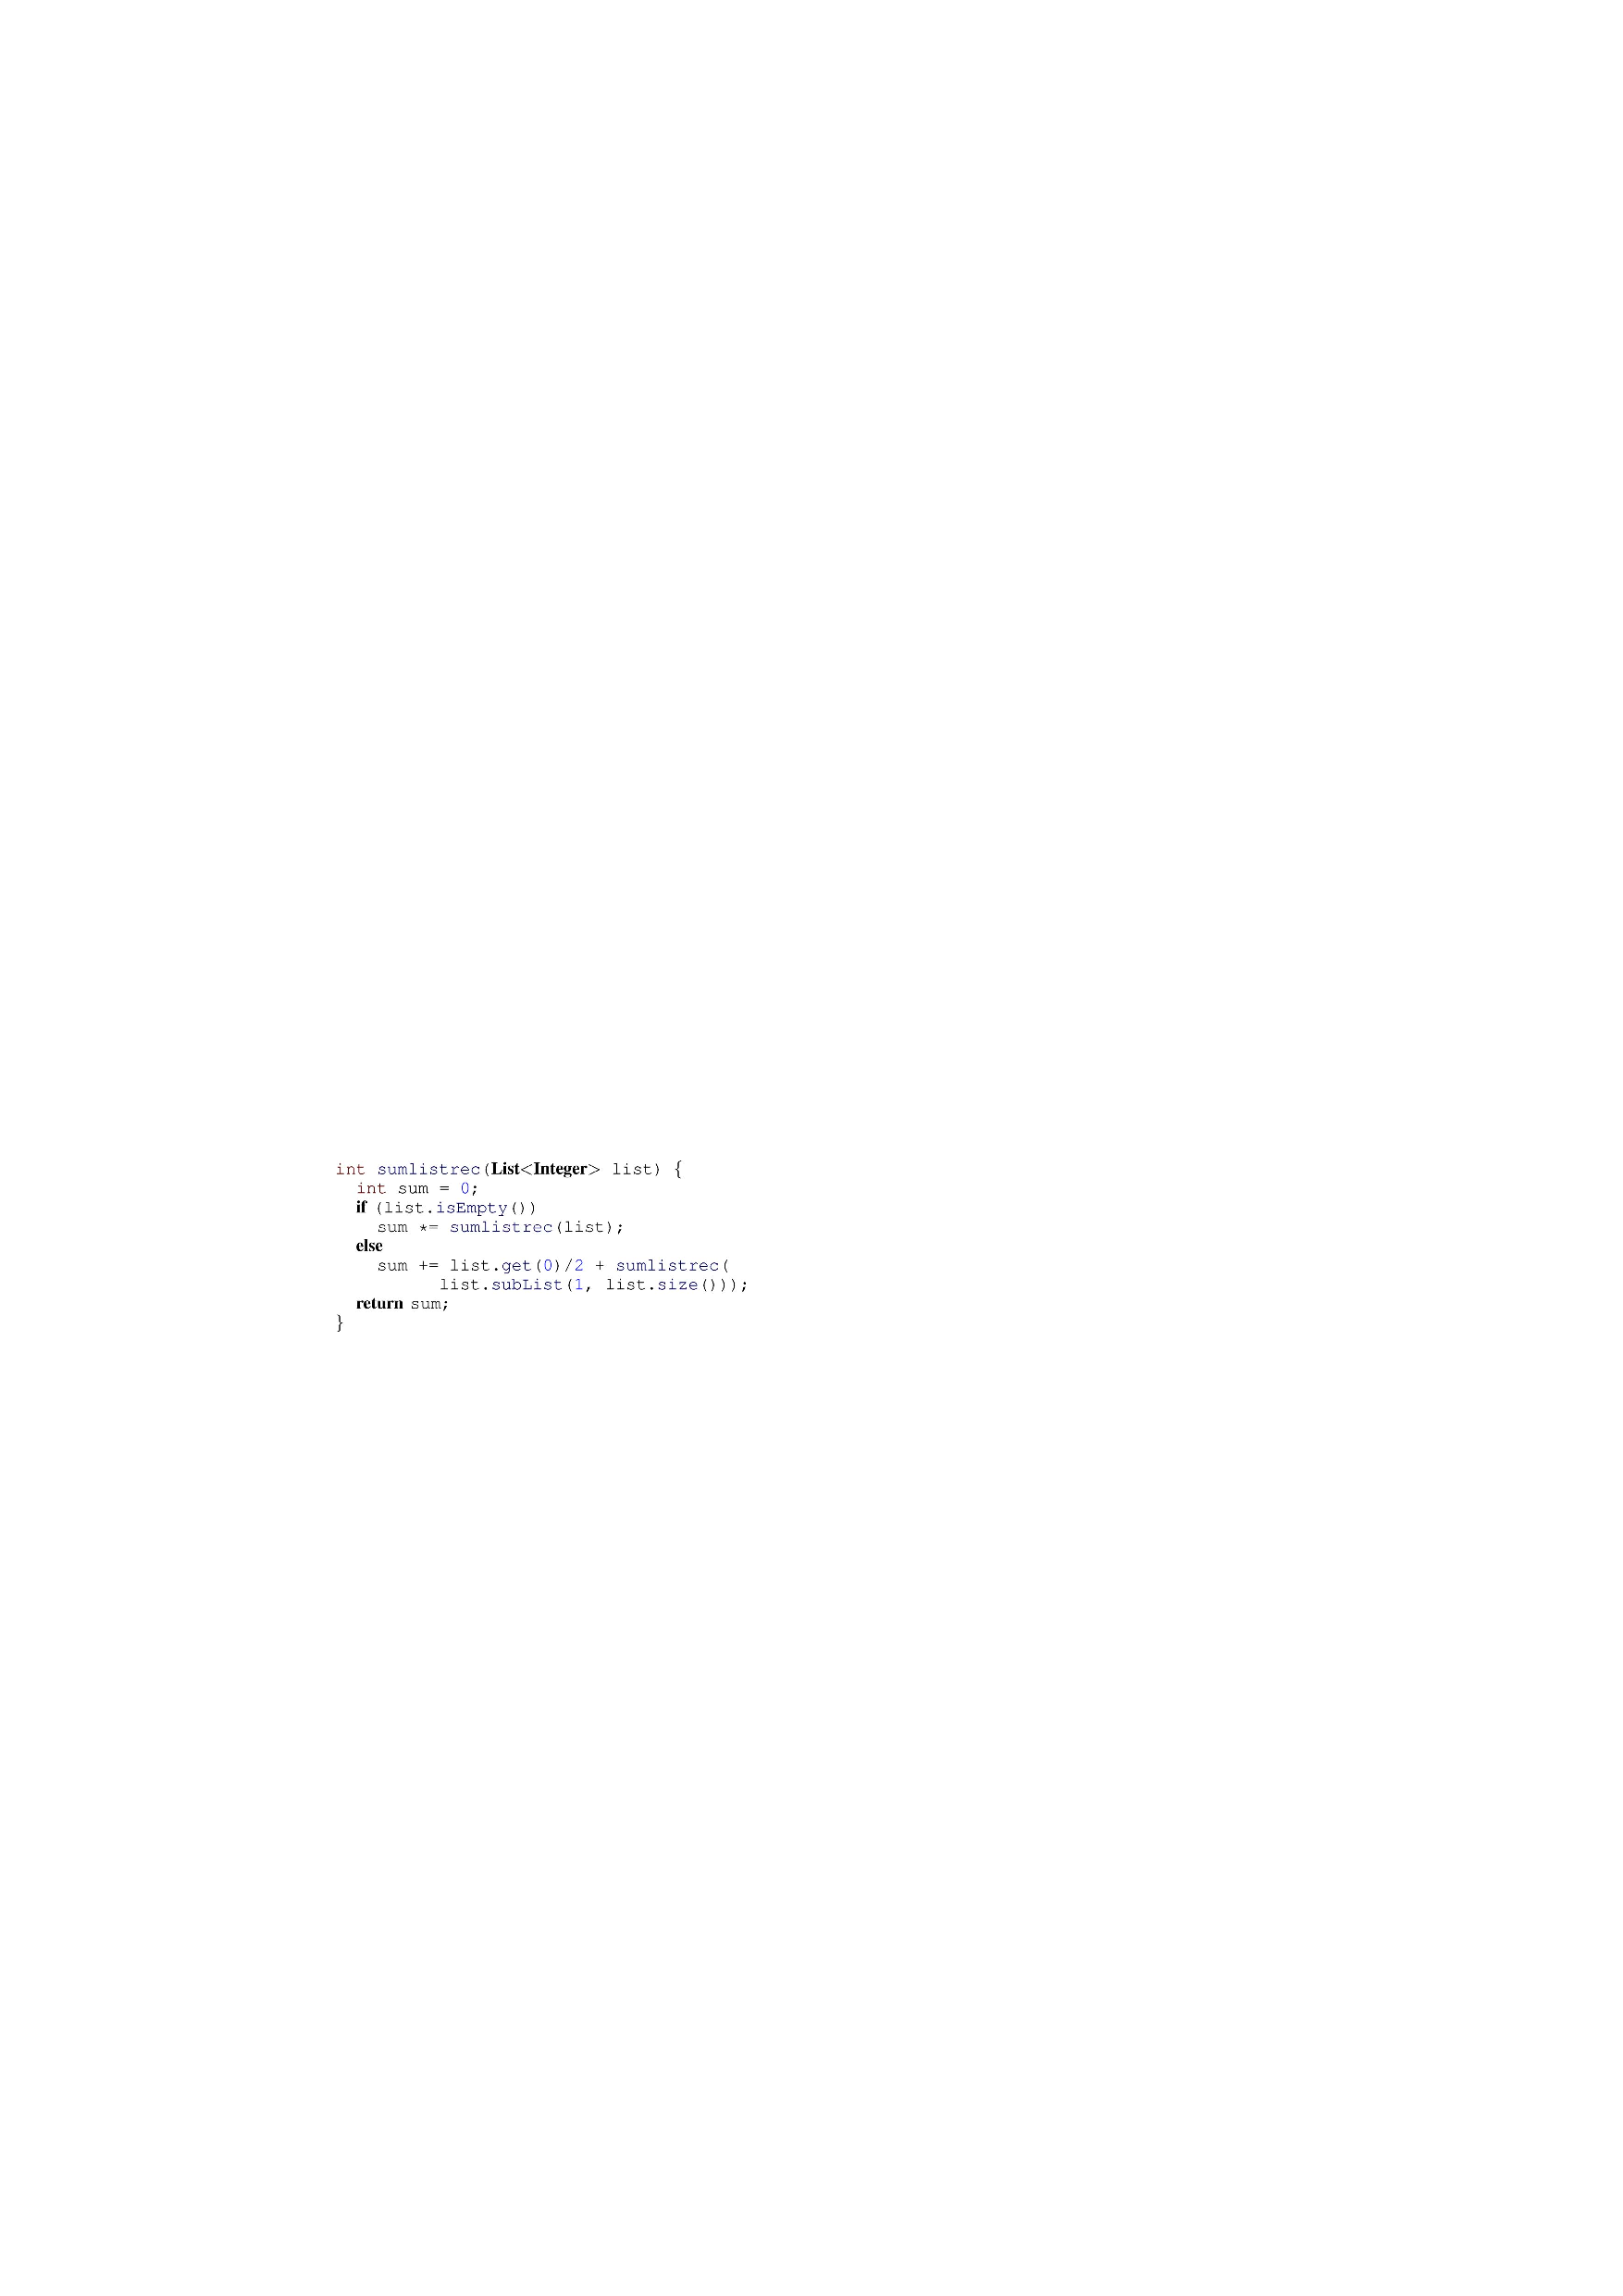
\psfig{file=infrec.pdf}
\caption{Initial population function, for array sum, that enters into infinite recursion in the if statement}
\label{initial rec}
\end{figure}

\begin{figure}
\centering
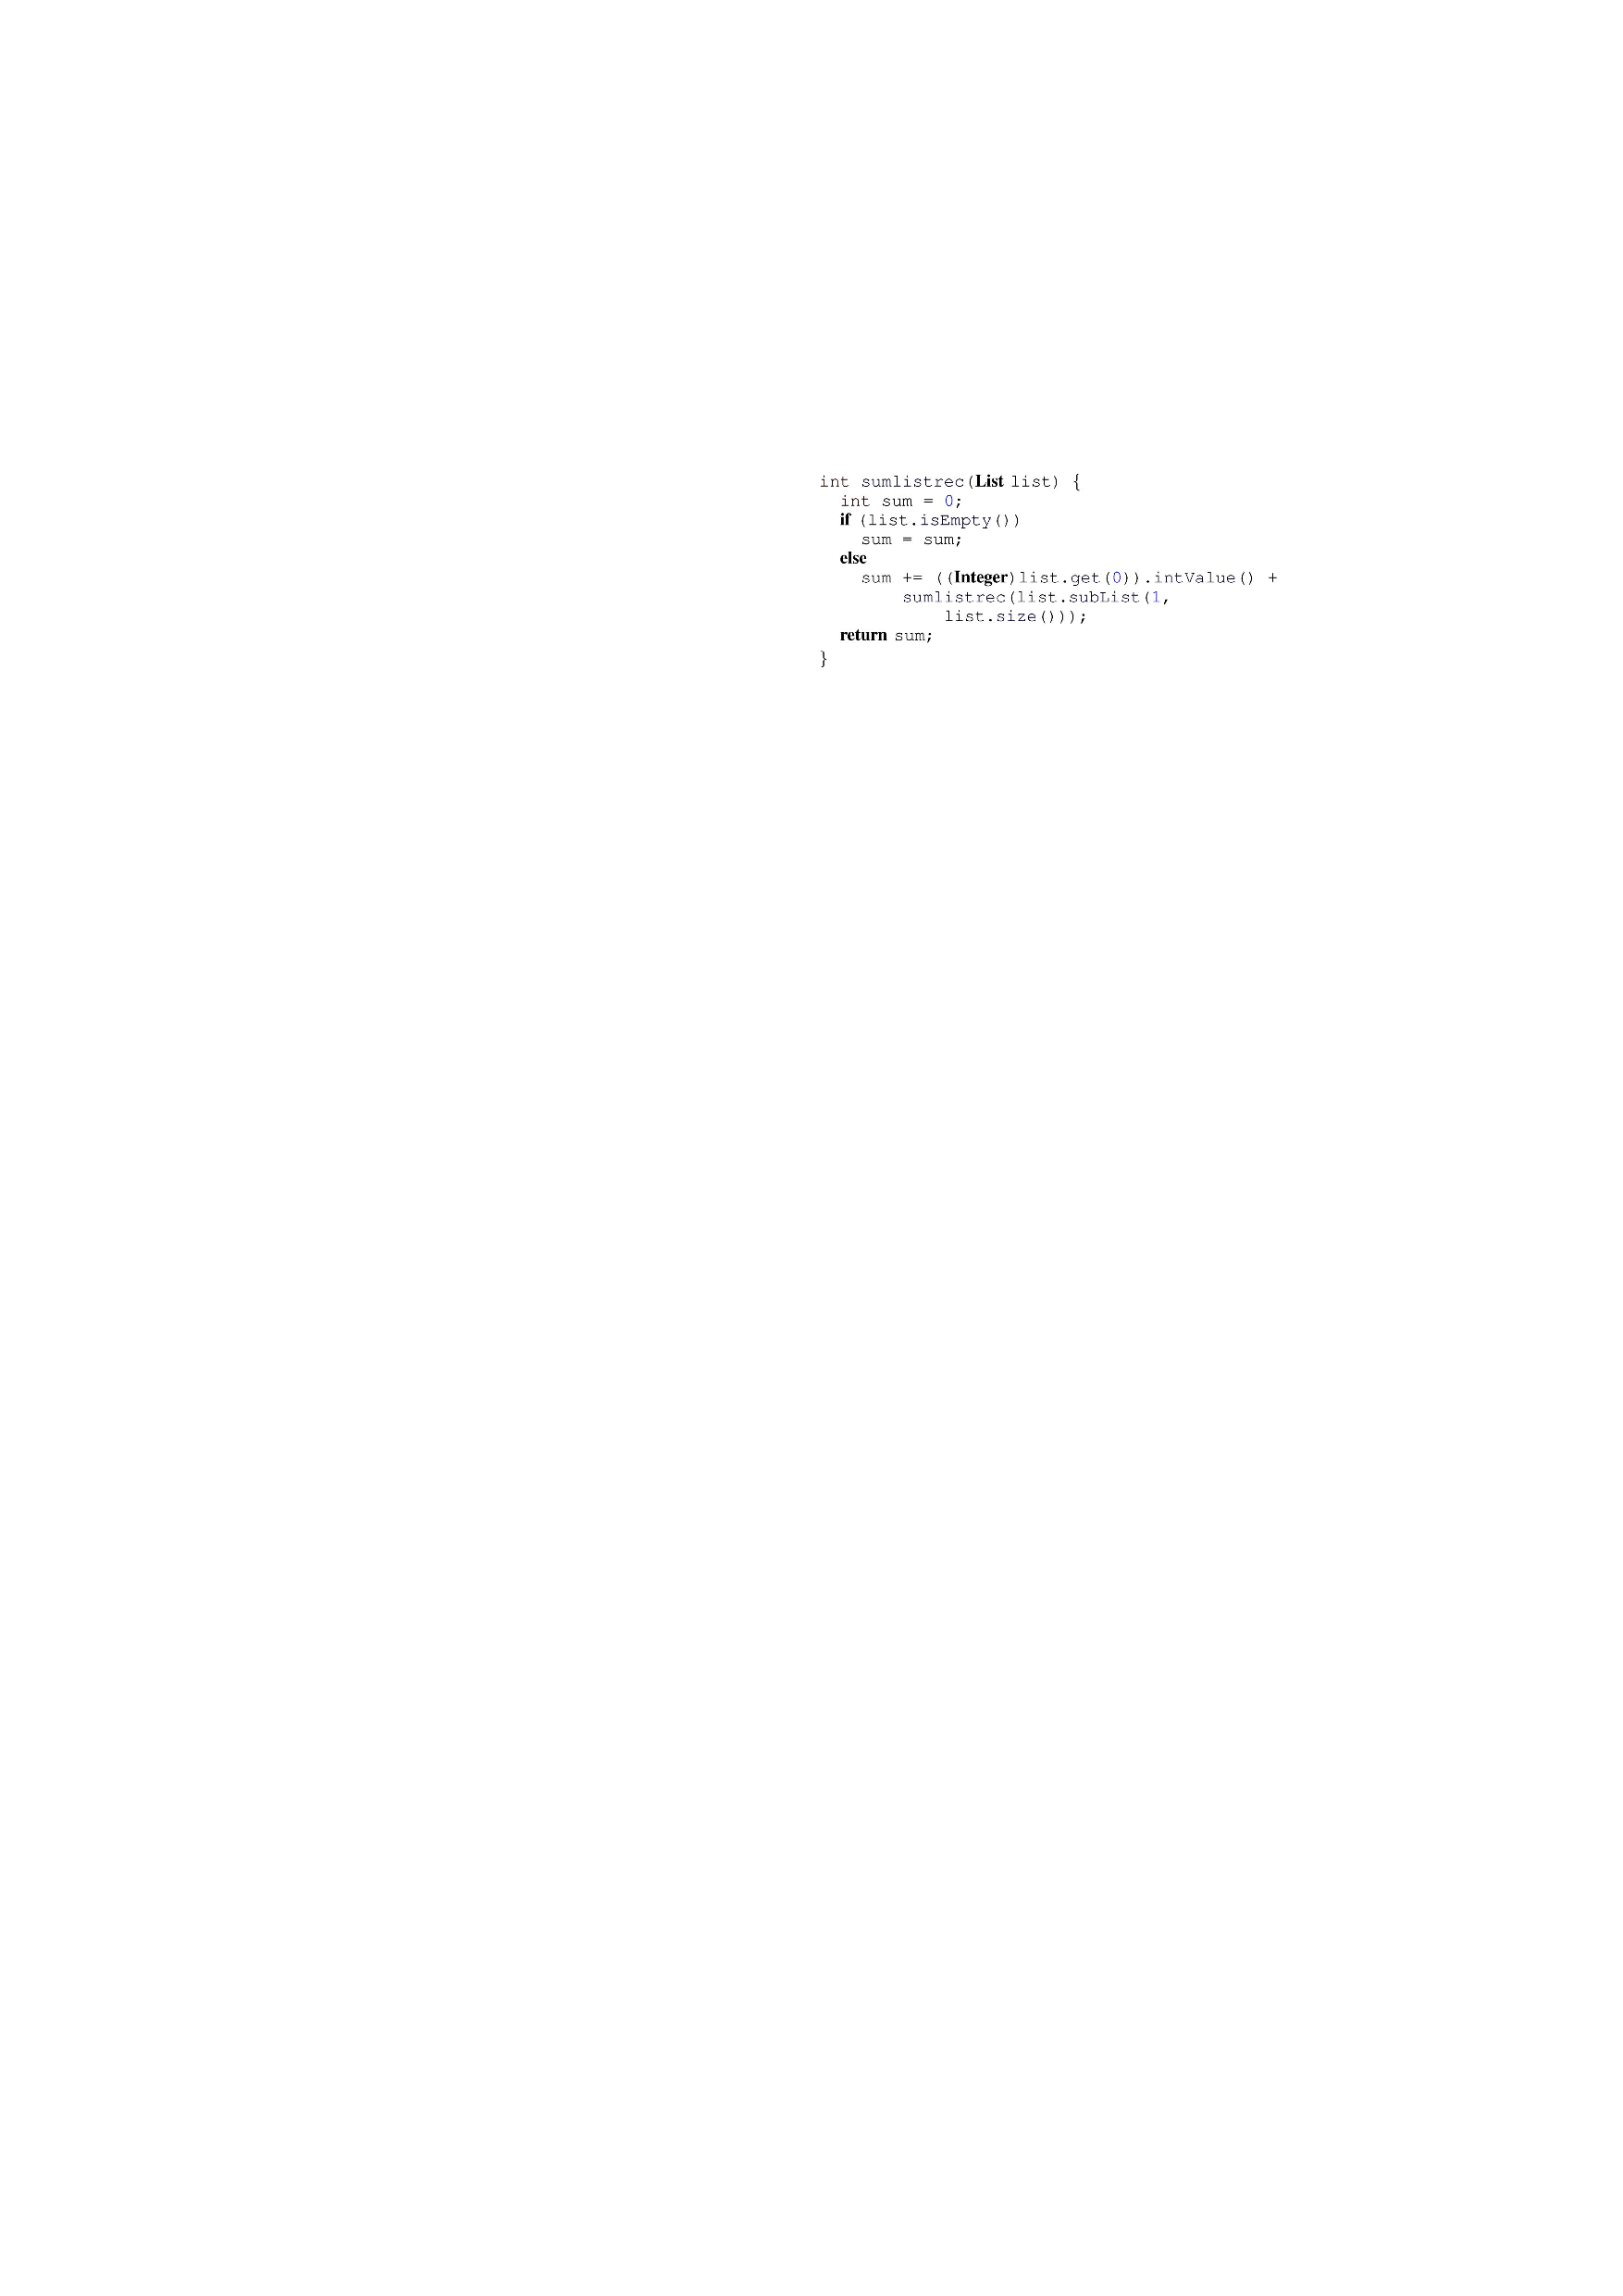
\psfig{file=recsolution.pdf}
\caption{FINCH's solution to the intial program presented in Figure~\ref{initial rec}}
\label{final rec}
\end{figure}

\subsubsection{Array Sum}
The array sum problem consists of adding up all the values in an array. This problem is important because it would require evolving a loop or recursion to solve it. This would show that FINCH is capable of evolving more complex programs\par
FINCH was able to produce a solution to this problem for both recursion and loops. This experiment showed that FINCH is able to evolve using different list abstractions such as List and ArrayList.

When evolving array sum with recursion the initial population consisted of an individual which entered infinite recursion as shown in figure \ref{initial rec}. Due to the way FINCH deals with non-halting programs this was not a problem and evolution was able to ensue. The resulting code from evolving Figure \ref{initial rec} is shown in Figure \ref{final rec}.


\subsection{Automated Bug Repair}

Schulte et al.,~\cite{Assembly:2010} were able to show that it is possible to fix human programming errors though bytecode and assembly. \cite{Assembly:2010} were able to successfully debug various programs containing bugs such as infinite loops and remote buffer overflows. The interesting thing about these experiments was that it was done on real programs with real bugs and at times the programs consisted of thousands of lines of code. Some of the bugs that they were able to fix through instruction-level code were not possible in their previous work~\cite{Forrest:2009} with source code. This shows that a wider array of bugs can be fixed by using instruction-level code.

Although a considerable amount of offspring with a fitness of zero were produced this did not seem to damage the result. The average number of fitness evaluations required to produce an offspring that passed all the tests was 63.6 for C,in previous work~\cite{Forrest:2009}, and 74.4 for assembly. This indicates that not much more computational work is needed to to evolve repairs in assembly. Even programs that contained thousands of lines of code only required a few runs. Thus, evolving programs in instruction-level code is feasible.
 

\subsection{Future Work}


Future work may include evolving programs whose solutions are much longer and complicated. Orlov et al.,~\cite{FINCH:2011} proved that by applying GP to bytecode it is possible to solve many simple problems. However, most of the problems only consisted of a small number of lines of code. It would be exciting to see something large and more complex be evolved. Also, as shown in Figure~\ref{final rec} a solution given by FINCH might not be very legible once decompiled back to source code. Refactoring would have to be done to make the code more readable and maintainable.

An extension of future work, using the research by \cite{Assembly:2010}, could include debugging on less focused areas. For example, attempting to fix bugs that require more fixes throughout the code; instead of one line. Also, there is the question of how applicable automated bug repair is in a real world situation. In most real world scenarios test coverage is very minimal and would rarely cover the entire code base.


\section{Conclusion}
There are things at the instruction-level that are a lot simpler to do than at the source code level. Things including evolving programs as a whole and reduced assumptions of the program being evolved by the EA.Also it is easier to deal with the semantic constraints if so desired. Schulte et al., and Orlov et al.,~\cite{Assembly:2010, FINCH:2011} showed that evolving instruction-level code is just as good as source code and at times even better due to the fact there some things that they have only been able to do at the instruction-level. In conclusion, evolving instruction-level is feasible and exciting for the field of EC since it opens up many possibilities that were once unavailable.
%\end{document}  % This is where a 'short' article might terminate

%ACKNOWLEDGMENTS are optional
\section{Acknowledgments}
Nic Mcphee, Elena Machkasova

%
% The following two commands are all you need in the
% initial runs of your .tex file to
% produce the bibliography for the citations in your paper.
\bibliographystyle{abbrv}
\bibliography{EricBibliography}  % ElenaSample.bib is the name of the Bibliography in this case
% You must have a proper ".bib" file
%  and remember to run:
% latex bibtex latex latex
% to resolve all references
%
% ACM needs 'a single self-contained file'!
%
%APPENDICES are optional
%\balancecolumns

\end{document}

\appendix
%Appendix A
\section{Headings in Appendices}
The rules about hierarchical headings discussed above for
the body of the article are different in the appendices.
In the \textbf{appendix} environment, the command
\textbf{section} is used to
indicate the start of each Appendix, with alphabetic order
designation (i.e. the first is A, the second B, etc.) and
a title (if you include one).  So, if you need
hierarchical structure
\textit{within} an Appendix, start with \textbf{subsection} as the
highest level. Here is an outline of the body of this
document in Appendix-appropriate form:
\subsection{Introduction}
\subsection{The Body of the Paper}
\subsubsection{Type Changes and  Special Characters}
\subsubsection{Math Equations}
\paragraph{Inline (In-text) Equations}
\paragraph{Display Equations}
\subsubsection{Citations}
\subsubsection{Tables}
\subsubsection{Figures}
\subsubsection{Theorem-like Constructs}
\subsubsection*{A Caveat for the \TeX\ Expert}
\subsection{Conclusions}
\subsection{Acknowledgments}
\subsection{Additional Authors}
This section is inserted by \LaTeX; you do not insert it.
You just add the names and information in the
\texttt{{\char'134}additionalauthors} command at the start
of the document.
\subsection{References}
Generated by bibtex from your ~.bib file.  Run latex,
then bibtex, then latex twice (to resolve references)
to create the ~.bbl file.  Insert that ~.bbl file into
the .tex source file and comment out
the command \texttt{{\char'134}thebibliography}.
% This next section command marks the start of
% Appendix B, and does not continue the present hierarchy
\section{More Help for the Hardy}
The sig-alternate.cls file itself is chock-full of succinct
and helpful comments.  If you consider yourself a moderately
experienced to expert user of \LaTeX, you may find reading
it useful but please remember not to change it.
%\balancecolumns % GM June 2007
% That's all folks!
\end{document}
